\section{Experimental Methods}
\subsection{Photon Beam}
** ToDo: Think about if/where to include the calculation of the ratio of knockout neutrons to fission neutrons.
Have only done calculation for Thorium.

A bremsstrahlung photon beam is produced by the passage of 10.5 MeV electrons through a 1" thick slab of aluminum.
Aluminum was chosen for a radiator because it has a neutron knockout threshold above the energy electron beam.
This ensured that the bremsstrahlung radiator was not a source of fast neutrons, which would have the potential to make their way into the experimental cell and cause false neutron events.
Downstream from the bremsstrahlung radiator, a sweeping magnet removes excess electrons from the photon beam (see figure~\ref{fig:Facility}).
Before reaching the experimental cell, photons are collimated by a series of polyethylene and lead collimators aimed at eliminating beam contaminants.
The energy distribution of photons reaching the target was assessed using an MCNP simulation that included the creation and collimation of Bremsstrahlung photons produced by a mono energetic electron beam incident on an Aluminum radiator.
The resulting energy distribution is shown in figure~\ref{fig:BremDist}.

\begin{figure}[h]
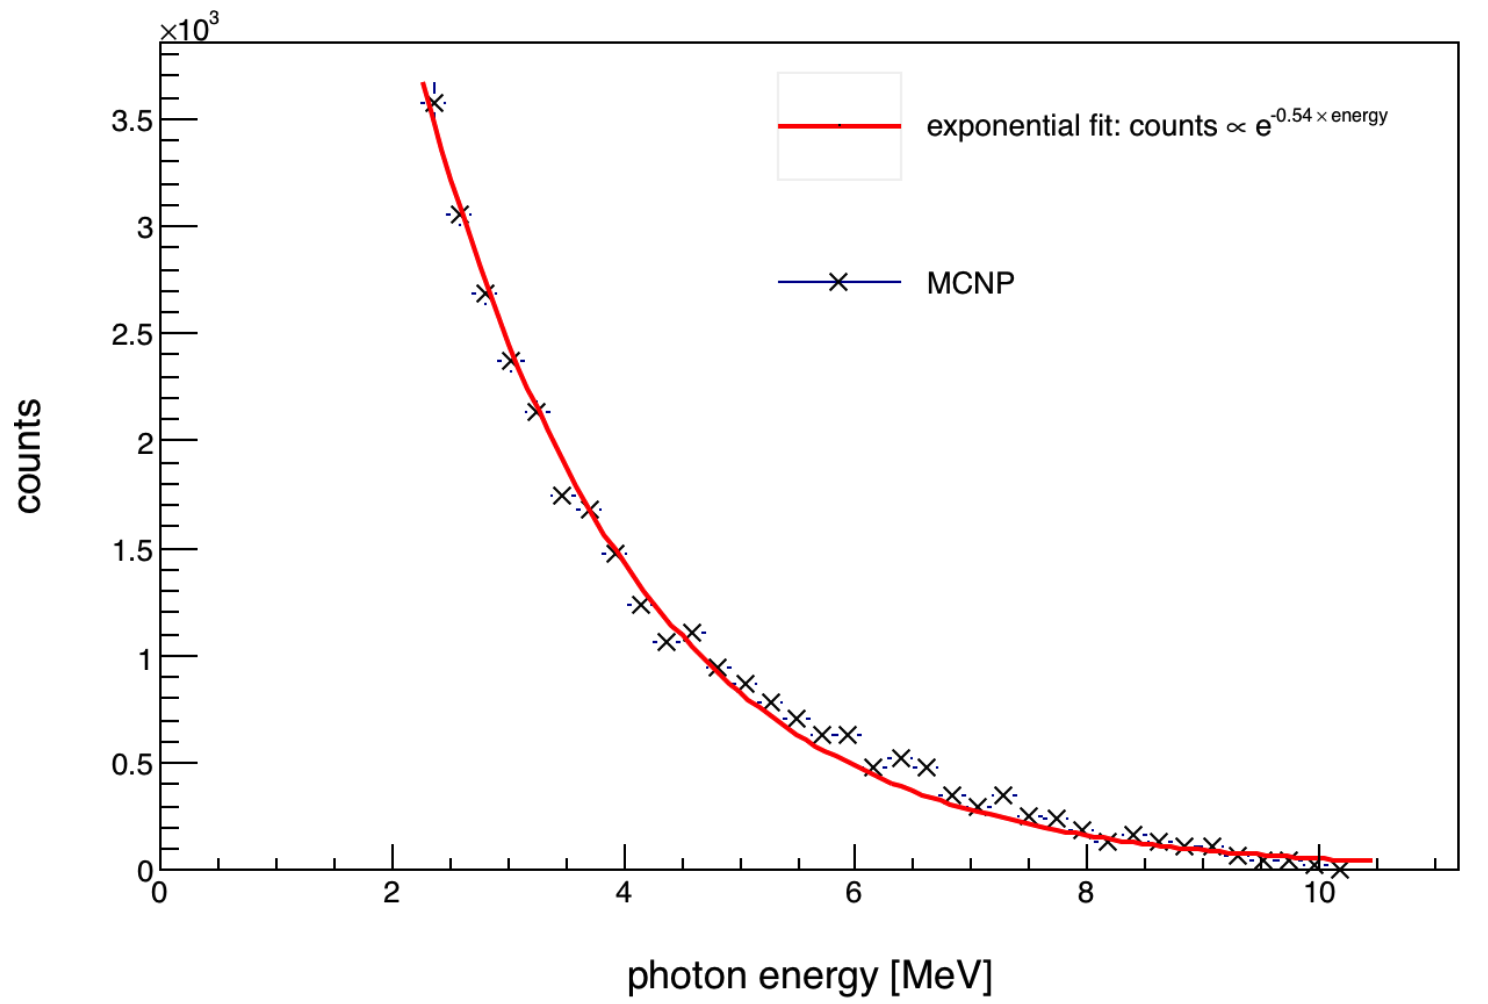
\includegraphics[width=0.9\textwidth]{Content/Methods/MCNPBremDistribution.png}
\caption{Result of an MCNP simulation of the energy distribution of the Bremsstrahlung photons that reach the target.
Points are from the simulation, and the line is an exponential fit ($Ae^{-bx}$).
The constant of proportionality, $A$, is arbitrary. The value for $b$ is 0.54.}
\label{fig:BremDist}
\end{figure}

When attempting a measurement of prompt neutrons from photofission, an ambiguity can arise between neutrons from photofission and neutrons from $(\gamma, xn)$.
This is because the two reactions have similar cross-sections within the GDR region.
Furthermore, there is significant overlap between the energy spectra of the neutrons from $(\gamma, xn)$ and from photofission.
Since this measurement is concerned only with observing two neutrons in coincidence, it suffices to set the Bremsstrahlung end-point at 10.5 MeV, since this value is below the ($\gamma, 2n$) threshold for of the targets, which is $\sim$12 MeV.
A 10.5 MeV end-point still leaves the possibility of the detection of multiple neutrons from ($\gamma, 1n$) in a single pulse, which is referred to as an accidental coincidence.
An \textit{accidental} neutron coincidence occurs when two uncorrelated neutrons are detected in the same pulse.
All accidentals follow the Poissonian distribution, and for this reason they can be subtracted from the data.
The details and justifications of this procedure are discussed in section~\ref{Subtraction of Accidentals}.

The electron pulse width was set to 3 ns and had a 1.1A peak current, with a repetition rate of 240 Hz.
The 3 ns pulse width is not a significant source of error in the measurements of neutron time of flight, since neutron events had a median time of flight of about 80 ns.
The accelerator current is set by requiring that there be, on average, fewer than one fission per pulse, thereby reducing the detection of uncorrelated neutrons from multiple fissions occurring in a single pulse.
Even so, the detection of uncorrelated neutrons is unavoidable because of statistical fluctuations.
To address this, a technique is developed to subtract these events from the data (see section~\ref{Subtraction of Accidentals}).

**ToDo Discussion about the LINAC's low duty factor??

\subsection{Particle time of flight determination}
\label{reconstruction}
%python file: ProductionAnalysis/TOFGraphs
\begin{figure}[htbp]
\begin{center}
\subfloat[$\Delta T$s with no target in place. ]{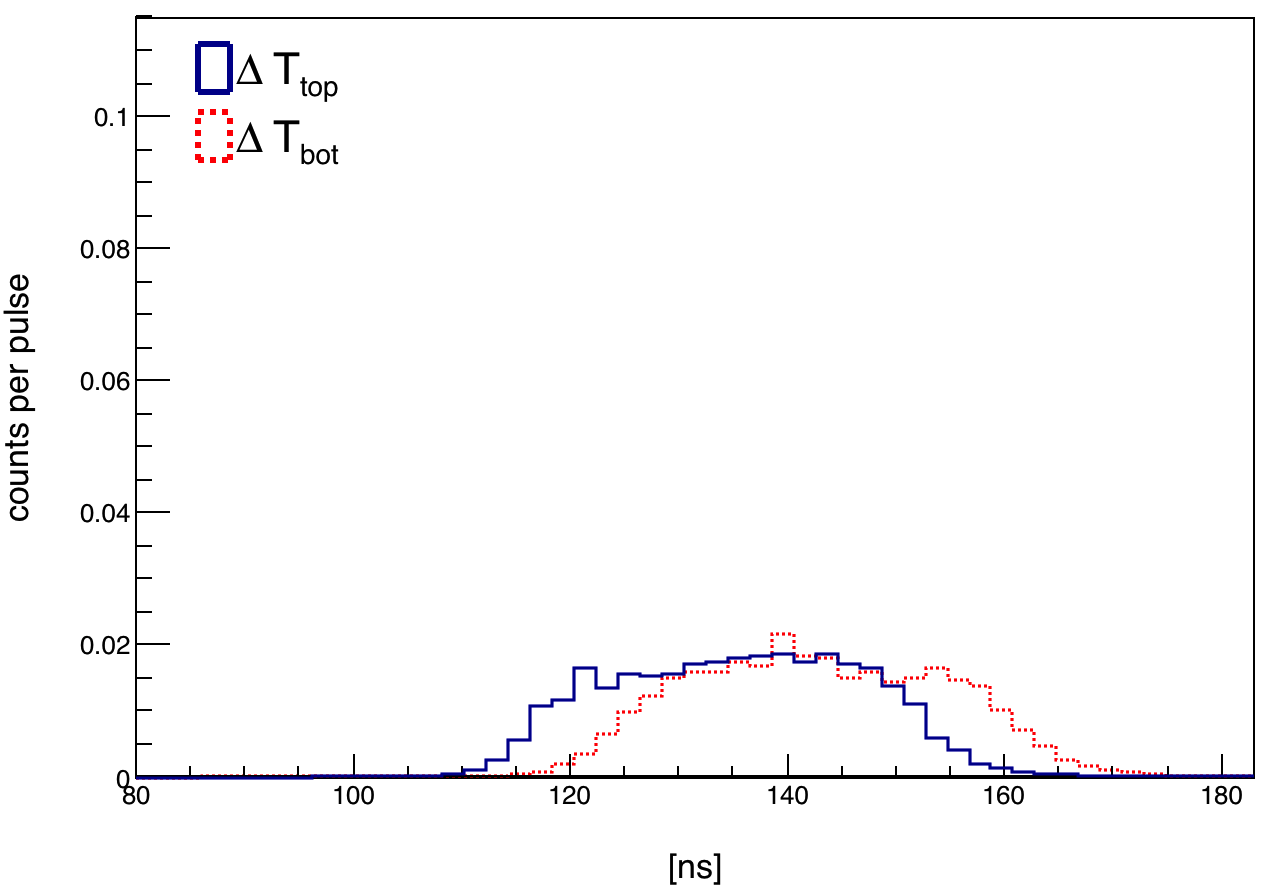
\includegraphics[width=0.5\textwidth]{Content/Methods/ToF0.png}}
\end{center}

\subfloat[$\Delta T$s with Aluminum target.]{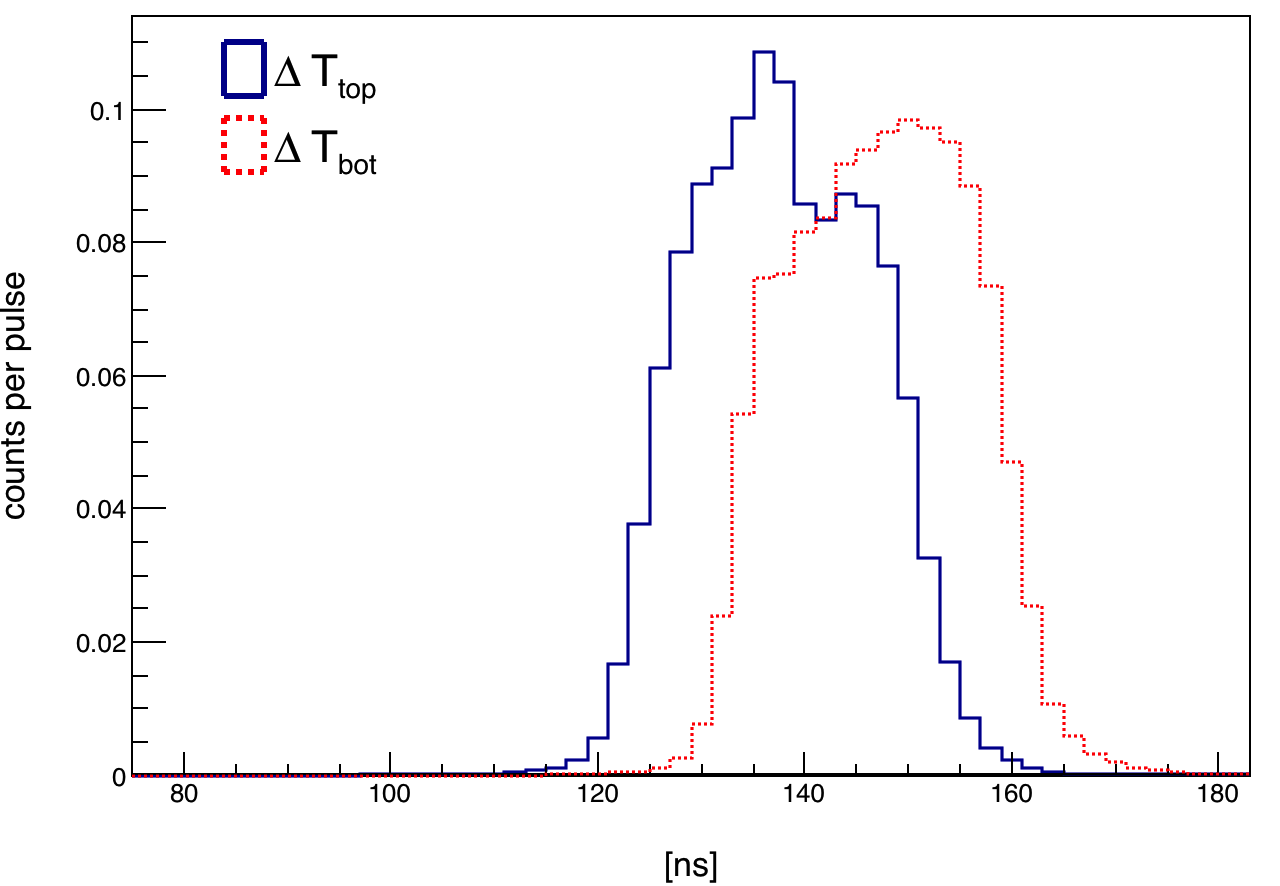
\includegraphics[width=0.5\textwidth]{Content/Methods/ToF1.png}}
\subfloat[Average of $\Delta T_{\text{top}}$ and $\Delta t_{\text{bot}}$  with Aluminum target in place.]{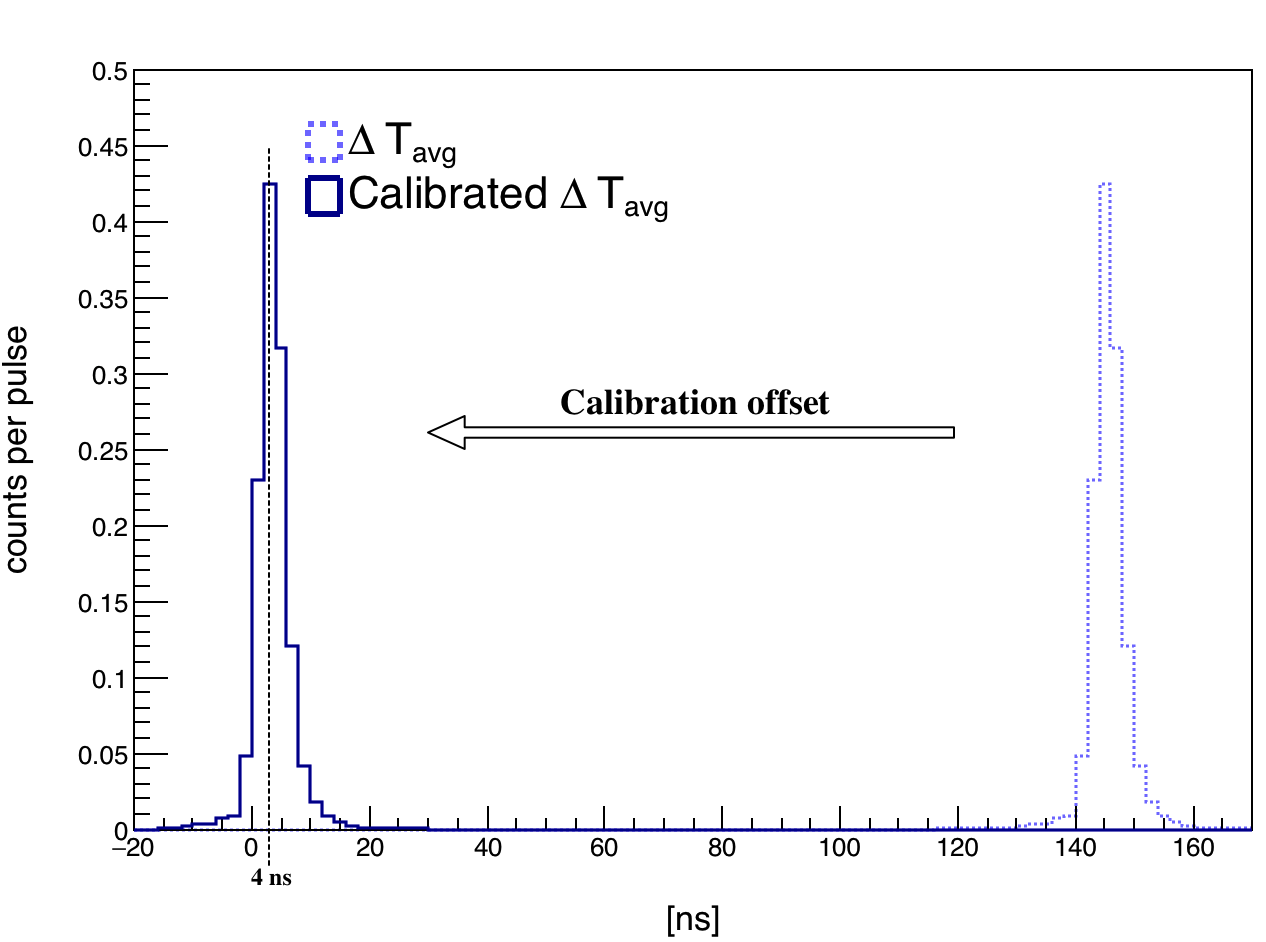
\includegraphics[width = 0.5\textwidth]{Content/Methods/ToF2.png}}
\caption{(a) $\Delta T$ spectra from each PMT of a detector with no target in place.
Despite the lack of a target, the beam dump does not collect all photons.
This background is caused by photons that scatter from various surfaces within the experimental cell.
(b) The introduction of a non-neutron producing target, made from aluminum, produces a peak caused by the scattering of photons from the target.
These photons have a constant time of flight, so the width of these spectra are reflective of the range of times taken for scintillation light to propagate from the points of scintillation to a PMT.
(c) Taking the average between the $\Delta T$s of the top and bottom PMT gives a sharper peak, since the sum of times from both both PMTs is reflective of the time required for light to travel the entire length of a detector, regardless of the location of the particle hit.
The correct timing offset can be now be found since the photons have a time of flight of 4 ns. }
\label{fig:ToFDetermination}
\end{figure}

Each scintillator was equipped with two PMTs, one fixed at each end of the scintillation cell, with the exception of the detectors located farthest downstream at $\pm30^{\circ}$ which had only a single PMT.
The PMTs provide a signal in response to scintillation light with a timing resolution of less than 1 ns.
However, the main source of uncertainly in the time of a particle hit is variation in the time taken for scintillation light to propagate to the PMTs. No pulse shape discrimination was used in this study.
Particle identification, along with the reconstruction of energy and position was achieved solely from the timing of signals from PMTs.
The time of each event in a PMT was measured relative to a signal provided by the accelerator at the beginning of each pulse, which is referred to as the \textit{beam gun}.

Time of flight (ToF), the time for a particle to travel from the target to the face of a detector, was used to distinguish between photons and neutrons, and to measure neutron energy.
The time of flight was calculated by taking the average between the times of signals from the top and bottom PMTs, and subtracting an offset determined from a calibration.
For the detectors located at $\pm30^{\circ}$, which have only one PMT, ToF is calculated from the timing of events from a single PMT.

The ToF of a particle that causes coincident events in both PMTs of a detector, obeys the following relationship:
\begin{displaymath}
ToF = C_i + \Delta t_{\text{avg}} 
\end{displaymath}
where $\Delta t_{\text{avg}} $ is the average between the timing from the top and bottom PMTs, and $C_i$ is a constant timing offset which is the same for every pulse.
The subscript on $C_i$ is used because the timing offset can be different for each detector.
Any process that produces a timing delay that does not change from pulse to pulse contributes to $C_{i}$.
Examples of this are the time required for photons to travel from the bremsstrahlung radiator to the target, the propagation of signals through the wires connecting the PMTs, and delays in the electronics for processing.

The time required for scintillation light to travel through the detector, from the point of scintillation to a PMT mounted at either end, can vary from 1 ns for particles that hit very close to a given PMT, to about 8 ns for particles that hit across the detector from a given PMT.
The sum of the times taken for scintillation light to travel to the top and bottom PMTs is just the time taken for the light to travel the full length of the detector, which is nearly a constant.
The rate at which light propagates along the length of a detector is dependant on speed of light in the material and the light's flight path.
The flight paths of detected scintillation light tend to be parallel to the long axis of the detector, because these paths are the shortest possible, and only the first signal from a PMT is accepted.
Therefore, in taking the average of the times in the top and bottom PMT, the time required for scintillation light to propagate through the scintillator is considered to be a constant offset.
However, because the light paths are not always perfectly parallel to the detector, there is some variation in scintillation propagation times.
This variation was measured using a $^{60}Co$ source.
The $^{60}Co$ source, which emits coincident back-to-back photons, is placed at several positions along the face of a lead shielded scintillator.
At each position, a small hole is drilled through the lead to give the $^{60}Co$ source a line-of-sight to a well-defined point on the scintillator.
Then, a high timing-resolution photon detector is placed next to the $^{60}Co$ source and used as a ``start'' trigger.
The times of signals from each PMT, taken relative to the start trigger, can be summed to give the time taken for scintillation light to propagate through the detector.
The results of the data can be seen in figures~\ref{fig:Co60Validation} and~\ref{fig:Co60ValidationProject}.
% **ToDo: Make a figure for the setup of the co60 calibration.
\begin{figure}[H]
    \centering
    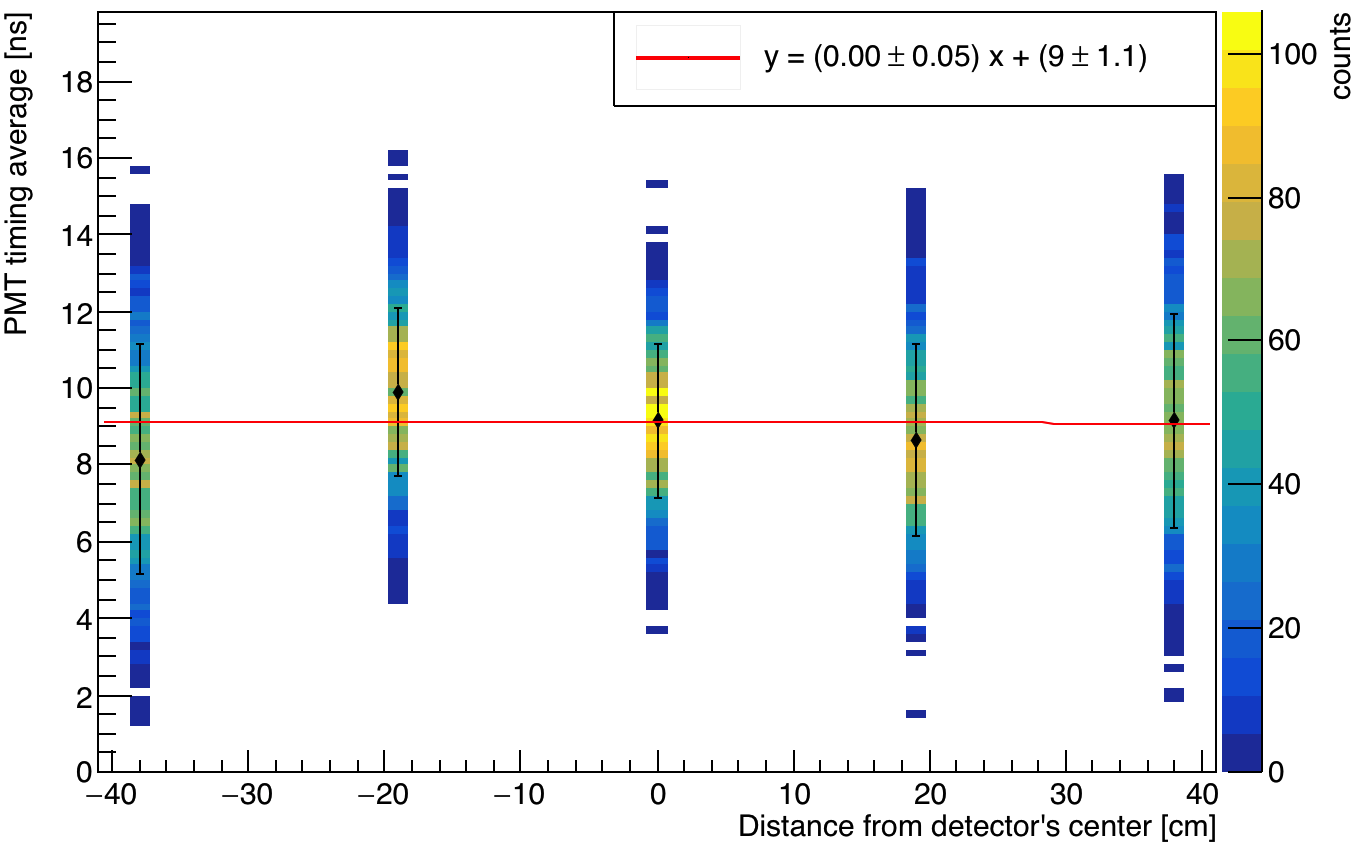
\includegraphics[width = 0.9\textwidth]{Content/Methods/CO60Validation.png}
    \caption{A $^{60}Co$ source, which emits coincident back-to-back photons, is placed at several positions along the face of a lead shielded scintillator.
    At each position, a small hole is drilled through the lead to give the $^{60}Co$ source a line-of-sight to a well-defined point on the scintillator.
    Then, a high timing resolution photon detector is placed close to the $^{60}Co$ source.
    When the $^{60}Co$ source decays, emitting two photons simultaneously, one photon is detected by the high timing-resolution detector serving as the ``start'' time, and the other scintillates in the detector being calibrated.}
    \label{fig:Co60Validation}
\end{figure}
\begin{figure}
    \centering
    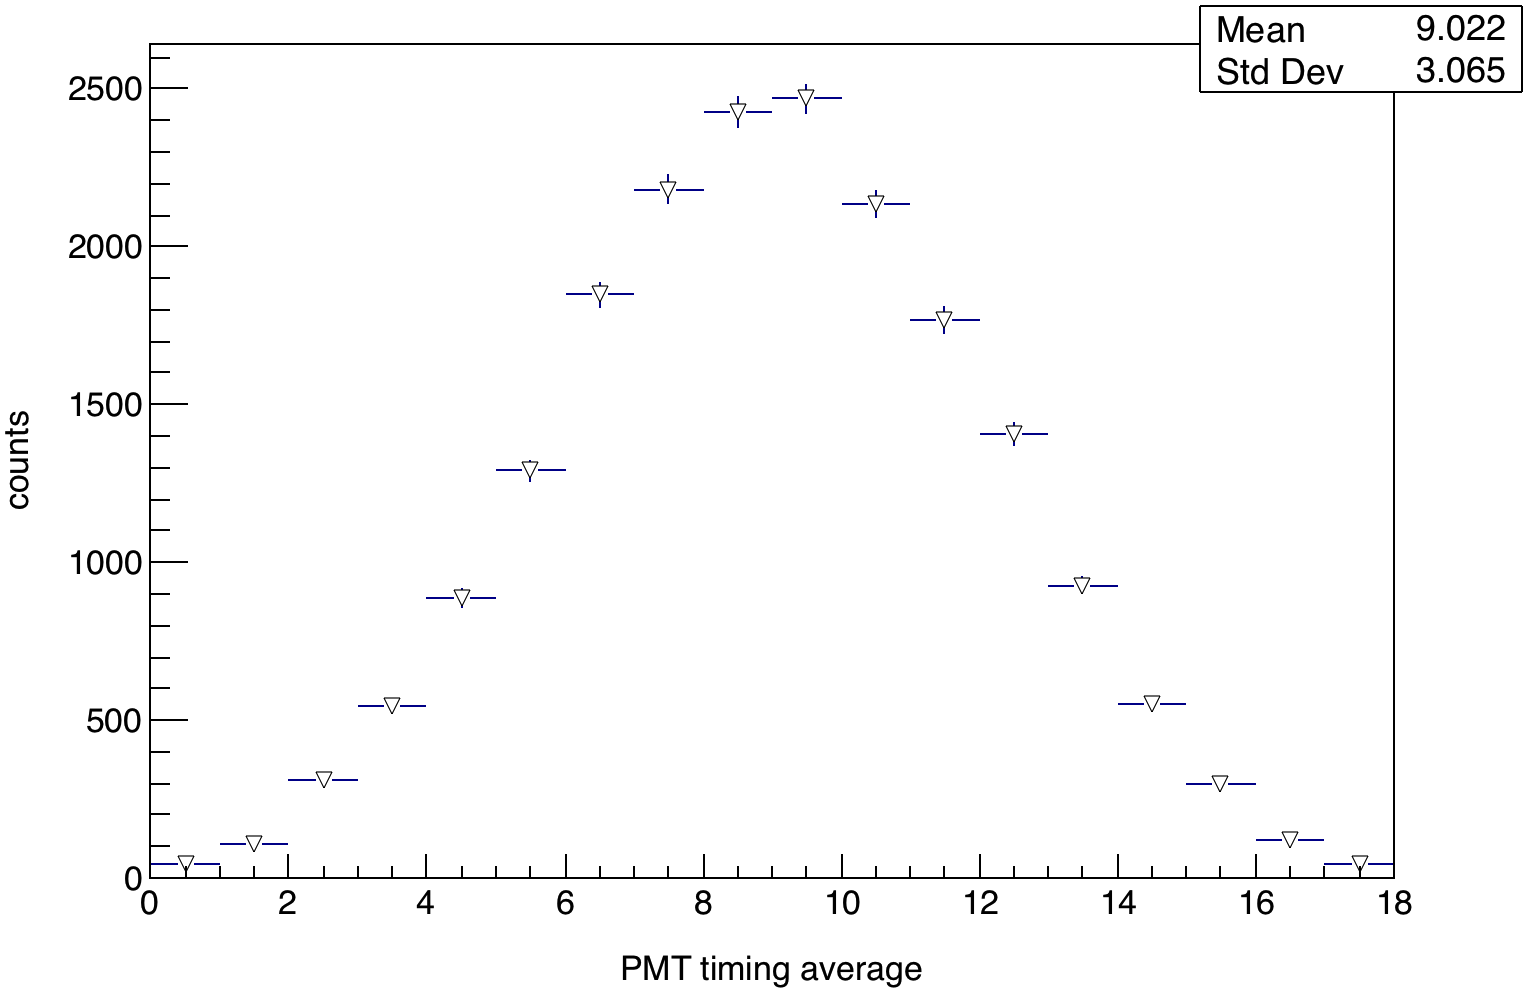
\includegraphics[width = 0.9\textwidth]{Content/Methods/CO60ValidationProject.png}
    \caption{Average of the times of coincident events in the top and bottom PMTs of a detector.
    These data, taken during the calibration of a detector using a $^{60}$Co source, are also shown in fig~\ref{fig:Co60Validation}, except here the data are projected onto the y-axis.
    The 3 ns standard deviation quantifies the variation in scintillation propagation times, which is a source of error in the measurement of time of flight.}
    \label{fig:Co60ValidationProject}
\end{figure}
%\begin{figure}
%    \centering
%    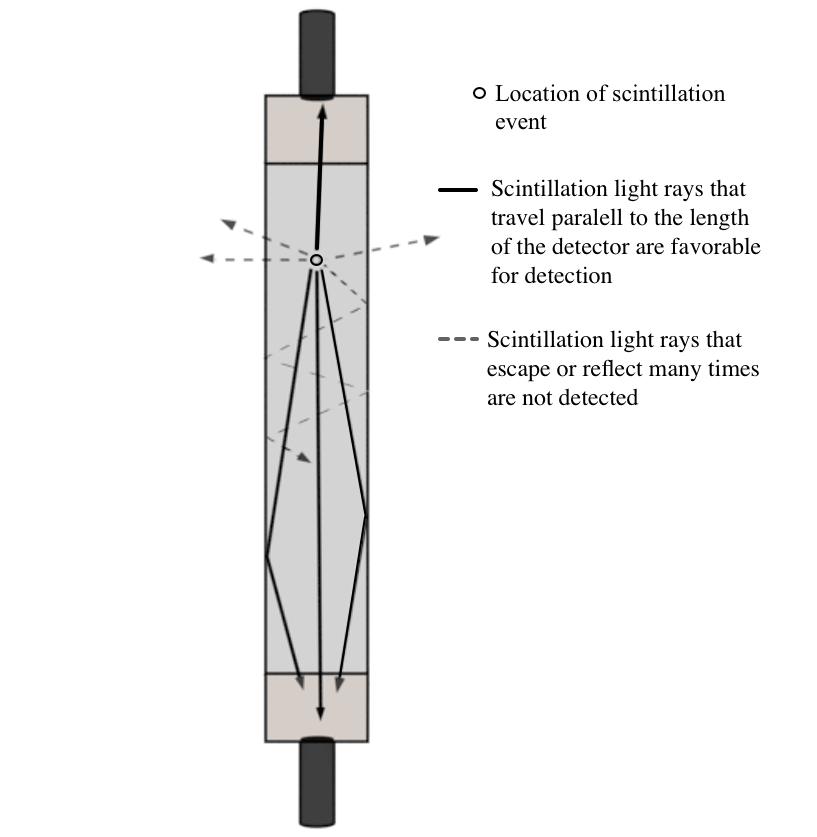
\includegraphics[width = 0.8\textwidth]{Content/Methods/lightpaths.png}
%
%    \caption{Hypothetical paths of light rays as they propagate through the scintillator after a scintillation event.
%    The light rays that first reach a PMT (solid) travel a shorter path than the others (dotted), and thus experience the least amount of attenuation.
%    This experiment always uses the first signal from a PMT and hence the data favors cases in which scintillation light travels a short path to a PMT.
%    In other words, the detectors favor the detection of scintillation light that is traveling parallel to the long axis of the detector.
%    As a result, the sum of the times required for scintillation light to reach both PMTs is just the time taken for light to travel the full length of the detector, which is a constant.
%    Thus, by taking the average time between coincident events in both PMTs, the time required for the propagation of scintillation light becomes a constant that is removed during calibration.
%    }
%    \label{fig:lightpath}
%\end{figure}
% Badness: The following paragraph could be better. 
The value of the constant offset for ToF calculation is determined by observing photons that scattered from the target.
Comparing the timing spectra of a non-neutron producing target made from aluminum, to the spectra produced when no target is used reveals a prominent peak caused by the scattering of photons from the target.
These photons must travel between 125 cm to 130 cm to reach a face of a detector, depending on whether the photons reach the detector near the center or at the edge.
It takes light 4.0 ns and 4.3 ns to travel 125 cm and 130 cm, respectively.
The difference between the two times is negligible for these purposes, so the ToF of photons that scatter from the target is assumed to be 4 ns.
With this assumption, the location of the photon peak in the timing spectra was used to calculate the offset in each detector.
   
\subsection{Particle Position Reconstruction}
% ToDo: The determionation of position could use a figure. The figure could indicate verticle reconstruction, and horizontal error. 
Spacial resolution in the horizontal plane is determined by the physical dimensions of the detector.
It's dimensions in the horizontal plane are comparatively small being 3.8x15 cm$^2$, so it suffices to use the geometric center of the detector as the horizontal component of a detected particle's position.
In doing this, a positional uncertainty of $\pm$7.5 cm is introduced, which expressed in terms of an angle is $\pm4^{\circ}$.
The final results of this work use an opening angle bin width of 20$^{\circ}$, so $\pm4^{\circ}$ is not large enough be a cause for concern.
The largest contributor to uncertainty in the reconstruction of particle position is the position in vertical direction, which is determined by the timing difference between signals in the top and bottom PMTs.

The determination of a particle's position in the vertical direction relies on the timing of coincident signals from both the PMTs of a detector.
The timing difference obeys a linear relationship with respect to the location of the particle hit along the length of the detector.
The z-coordinate will hereafter refer to a particle's position along the vertical axis, where $z=0$ corresponds to the geometric center of the detectors.

As discussed before, detected scintillation light tends to take fairly direct paths to the PMTs, experiencing few reflections off the boundary of the scintillation cell.
As a result, the timing difference between signals in the top and bottom PMTs is proportional to the difference in path lengths that the scintillation light must travel to reach each PMT, which is in turn proportional to the z-coordinate of the particle hit.
The exact linear relationship is determined through calibration by using collimated photons from a $^{60}$Co source.
Calibration is achieved by measuring the PMT top-bottom timing difference while the $^{60}$Co source is fixed at five different locations along the detectors length.
The setup for calibration was discussed in section~\ref{reconstruction}.
The result is shown in figure~\ref{fig:PMTDifference}.

\begin{figure}
    \centering
    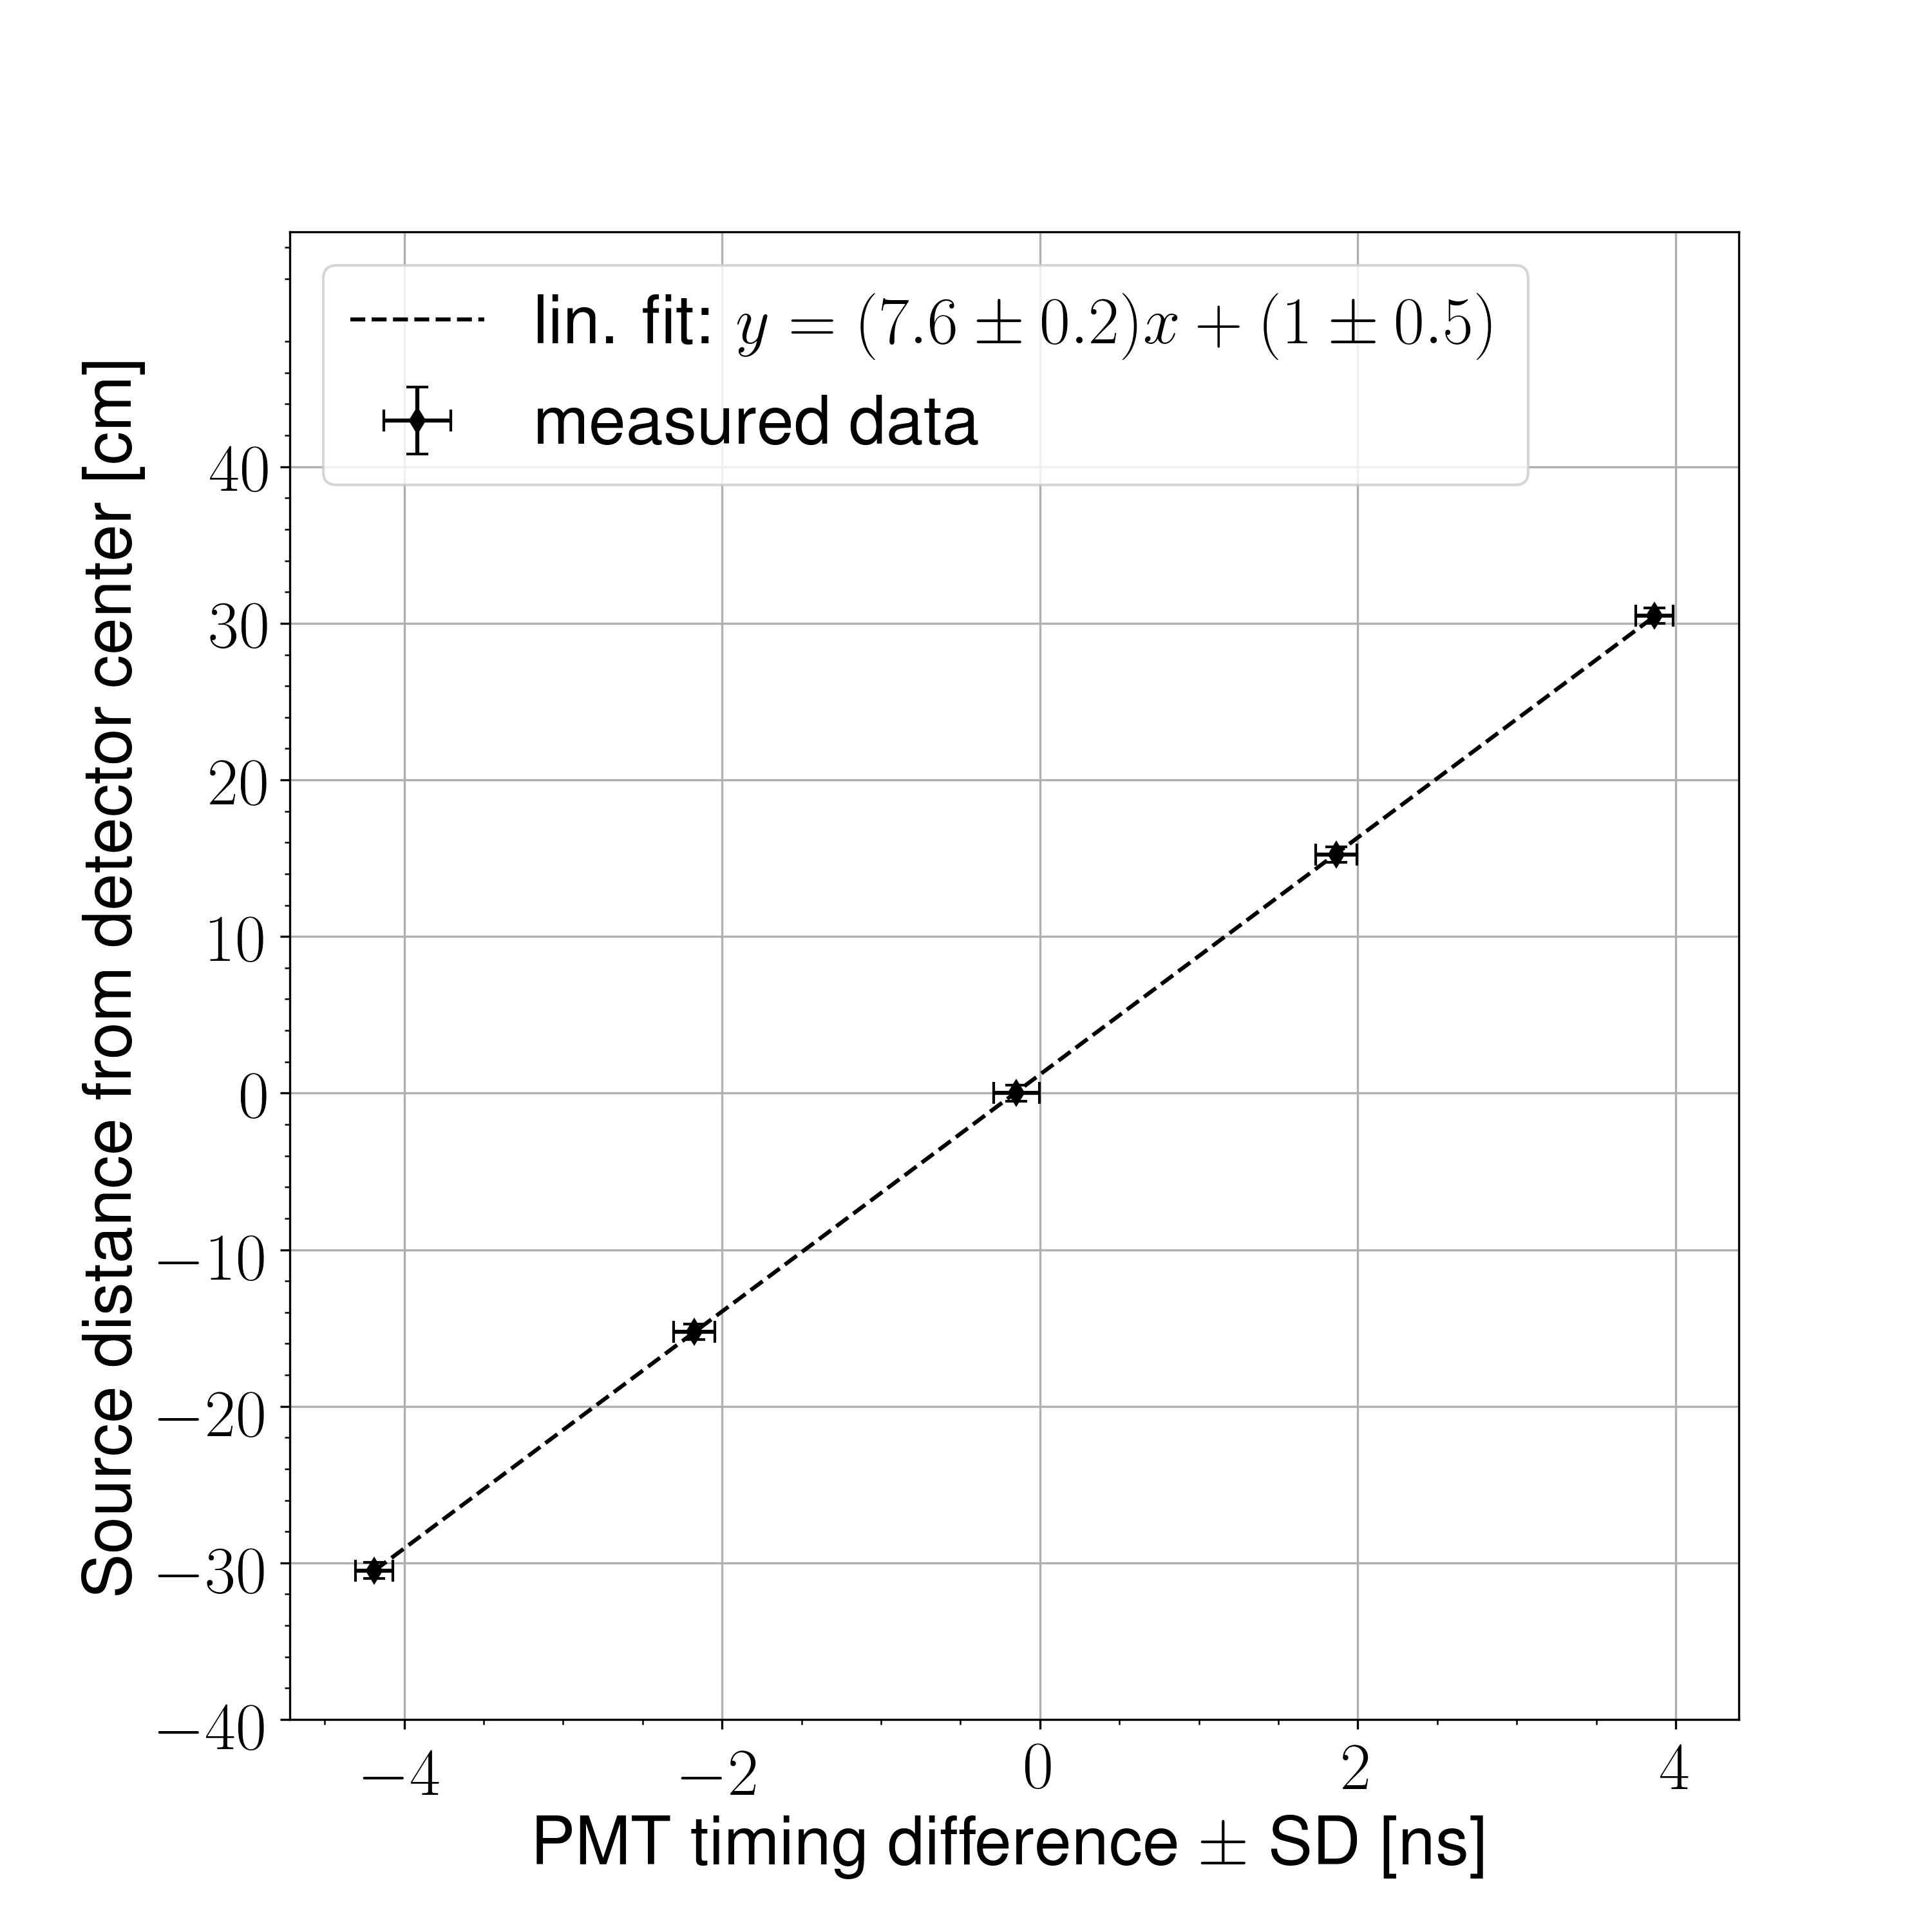
\includegraphics[width = 0.9\textwidth]{Content/Methods/PMTDifference.png}
    \caption{A collimated $^{60}Co$ source is used to produce events at precise locations on the detector.
    The particle's position along the detector's length is shown to vary linearly with respect to the timing difference between events in the top and bottom PMTs of a detector.}
    \label{fig:PMTDifference}
\end{figure}
\subsubsection{Detector Shielding}

The detector's shielding was designed with the aim of reducing cross-talk, the detection of photons, and noise.
The front face of the detectors, which face towards the target, are subject to the highest flux of gammas due to the scatting beam photons from the target.
The detection of a gamma renders a detector ``dead'' during the time in which fission neutrons reach the detectors.
Lead readily attenuates gammas, but has the side effect scattering neutrons.
If a neutron scatters prior to being detected, the ToF calculation will be incorrect because the neutron traveled an unknown distance to the detector.
The extent to which neutron distances of travel are perturbed due to scattering from lead shielding was quantified using an MCNP.
% ToDo: Add figure of neutron distances.
Accordingly, 1" of lead was placed along the front face of the detectors.
This effectively diminished gamma detection rates and, according to the simulation, is expected to cause negligible levels of neutron scattering.
Additional lead was used in some special areas that had high gamma flux: at the sides of detectors adjacent to the beam, and along the front faces of the detectors farthest downstream.

Placing lead behind the detectors was avoided in consideration of an MCNP-POLIMI simulation, which indicated that lead placed here facilitates cross-talk. \textit{Cross-talk} is an undesirable phenomenon in which a particle causes a hit in one detector, and then by any means (e.g. scattering), the same particle causes a hit in a different detector.
If both hits occur within the time frame typical for neutrons, then the cross-talk event cannot be distinguished from a true neutron coincidence.
Because cross-talk events are in fact correlated, they cannot be removed in analysis by the subtraction of accidentals.

\subsection{Detector Cross-talk}
%**ToDo: Expand this section. Graphs and a more detailed discussion. The cross-talk plot on the wiki could be insightful.
The geometry of the neutron detector array makes it kinematically impossible for a neutron to scatter from a proton in one detector--which is the basis for scintillation--then travel straight to another detector.
Rather, it is kinematically required that the neutron scatter from at least one intermediate nucleus while traveling between detectors.
This fact, which can be derived from simple two-body kinematics, shows that cross-talk is a "second-order" effect, because the neutron has to scatter from an intermediate nucleus, AND be detected in another detector.
However, the kinematics alone are not sufficient to neglect the effect of cross-talk, because the detectors and their shielding contain significant levels of carbon, lead, and other nuclei which could function as intermediate scattering points.
To address this, a detailed MCNP-POLIMI simulation was performed that modeled the entire neutron detector array, shielding, supporting structures, and the experimental cell.
Neutron detection physics was modeled by calculating the amount of energy converted into scintillation light, but did not include the propagation or detection of scintillation light.
The energy of scintillation slight is given in MeV equivalent electron energy (MeVee), which is the light output given by 1 MeV fast electrons.
For neutrons detected by elastic scattering on hydrogen, the light output is given by
\begin{displaymath}
L = 0.0364 E_n^2 +  0.125 E_n
\end{displaymath}
, where E is the energy deposited, equal to the change in kinetic energy.
Neutron interactions with carbon are assumed to generate a small light output equal to
\begin{displaymath}
L = 0.02 E_n
\end{displaymath}
% ToDo: Cite this from the MPPOST manual.
A distinct feature of MCNP-POLIMI, which is not included in the standard MCNP release, is its ability to model a $^{252}$Cf spontaneous fission source that emits neutrons with the correct correlations.
The detection rate of correlated two-neutron events, relative to the rate of detected cross-talk events, is found by tracking fission neutrons individually through the geometry.
In the simulation, coincident events were detected at a rate that is 36 times greater than for cross-talk events, which is less than a 3\% effect.
Accordingly, no attempt was made to correct for cross-talk in the final result.
% ToDo: Elaborate on the cross-talk simulation.

\subsection{Targets}
A depleted uranium (DU) target with dimensions of 4x2x0.05 $\text{cm}^3$ was used as the primary target for the measurement of two-neutron correlations.
DU received the majority of the allotted beam time because it is an even-even nucleus, and as a consequence fission fragments are emitted with a high degree of anisotropy.
One consideration for the design of the target is the rate of neutron scattering in the target.
This is a cause for concern because the neutron's direction of the travel is altered by scattering, which creates two-neutron opening angles that are not reflective of the opening angle immediately after fission.
While this effect cannot be completely eliminated, the target must be small enough such that neutron scattering can be neglected.
This issue is addressed by performing an MCNP simulation in which neutrons with an energy spectrum typical of fission neutrons are sampled uniformly within a target.
% ToDo: Expand on this section. Further discuss the MCNP simulation and add a relevant plot.
In the simulation, the probability that a neutron produced in the target escaped without scattering, was 97.5\%.
Because two neutrons are required for the formation of an opening angle, the rate of data contamination due to scattering is $(1-.975^2)$, or 5\% of two-neutron events.

It is desirable to have a target with symmetry that is consistent with the cylindrical symmetry of the neutron detector array.
To accomplish this, a thin rectangular target was rotated slowly about the vertical axis during data acquisition.
By doing this the cylindrical symmetry is preserved, since the measurement is reflective of an average of events which occurred while the target was at orientations from 0 to 2$\pi$.
This eliminates potential biases caused not by physics, but instead by the asymmetrical structure of the target.

\subsection{Measurements with $^{252}$Cf}
%ToDo: reread this and revise. Maybe place result and comparison of Cf measurements here instead of in results?

Opening angle measurements were also performed on neutrons from the spontaneous fission of $^{252}Cf$.
The configuration for this measurement was different than that for photofission measurements, as the photon beam can no longer be used for the timing ``start'' trigger.
The trigger for $^{252}$Cf consisted of two high timing-resolution scintillation photon detectors, with one fixed below and the other above the source at a distance of 15 cm.
With a coincidence window of $\Delta t\leq 4$ ns, 2-fold coincidence between both the photon detectors served as the timing start trigger.
Aside from the mechanism for a start trigger, the measurement methods for the $^{252}$Cf source are equivalent to those for photofission.

As opposed to the measurement of neutrons from photofission, when using neutrons from $^{252}$Cf, there is no concern of accidental neutron pairs.
Given the strength of the source, it is extremely unlikely for two fissions to occur during the neutron time of flight window, thus all detected neutron pairs are expected to be correlated.
Another difference between the two measurements is the clean and sharp peak produced by fission photons from $^{252}$Cf, compared to the increased smearing of the peak produced by photons scattering from the target during the photofission measurement.
In both measurements, this photon peak is used as a reference point for the time of flight of neutrons, so $^{252}$Cf has less error due to photon peak smearing.
The same normalization technique is used for both measurements, in which a correlated distribution is divided by the uncorrelated distribution of neutron pairs taken from different fissions.
Past measurements of the opening angle distribution of neutrons from the spontaneous fission of $^{252}$Cf are in good agreement, and thus are used as a benchmark measurement for this study.

